% -----------------------------------------------------------
%
%  CHAPTER 4  of Quantum information with atoms and photons
%
%  written by many authors Jan 2023
% -----------------------------------------------------------



The structure of the energy levels of a given atomic system can be different according to the resolution adopted to resolve it and which type of interactions have been considered. In particular, three structures are present: 

\begin{table}[h!]
\centering
\begin{tabular}{c|c|c|c}
\toprule
 $~$ \textbf{Structure} $~$  & $~$ \textbf{Energy} $~$ & $~$ \textbf{Frequency} $~$  & $~$  \textbf{Source} $~$ \\
\hline
\textit{Gross} & 1-10 eV & \makecell{$>$ 200 THz \\ (visible light)} &\makecell{nucleus-electron interaction \\ electron-electron interaction \\ and kinetic energy} \\ %\hline
\textit{Fine} & 10$^{-3}$-$10^{-2}$ eV & \makecell{$\sim$  1 THz \\ (far infra-red)} & \makecell{spin-orbit interaction \\ (relativistic effect)}\\ %\hline
\textit{Hyperfine} & 10$^{-6}$-$10^{-5}$ eV & \makecell{$\sim$ 1 GHz \\ (micro-wave)} & \makecell{magnetic dipole coupling \\ (nucleus-electron magnetic \\ interaction)} \\
\bottomrule
\end{tabular}
\caption{Atomic energy structures whit typical energies, frequencies and source of the spectra. }
\label{tab:en_lev}
\end{table}

In the following, only the first two structures are considered.

\section{From the Hydrogen atom to the Alkali}

An \textit{hydrogenoid atomic system} (which includes hydrogen atoms and Alkali atoms) is made of two elements:
\begin{itemize}
    \item a heavy attractor (the nucleus and the electrons of the inner shell) characterized by a mass $m_H$ and a momentum $\vec{p}_H$; 
    \item a light attractor (the outer electron) characterized by a mass $m_e$ and a momentum $\vec{p}_e$. 
\end{itemize}
The Hamiltonian of the system is 
\begin{align}
    H = \frac{\abs{\vec{p}_H}^2}{2 m_H} + \frac{\abs{\vec{p}_e}^2}{2 m_e} + V(\abs{\vec{r}_H - \Vec{r_e}}), 
    \label{eq:Hatoms1}
\end{align}
Where the first two terms are the kinetic energies of the heavy and light attractors, while the potential depends only on the modulus of the distance between them (radial potential).
Moreover, for $\vec{r}_H$, $\vec{r}_e$, $\vec{p}_H$ and $\vec{p}_e$
\begin{align}
    [({r}_H)_j,({p}_H)_k] &= i \hbar \delta_{jk}, \label{eq:comm1} \\
    [({r}_e)_j,({p}_e)_k] &= i \hbar \delta_{jk}, \label{eq:comm2} \\
    [({r}_e)_j,({p}_H)_k] &= [(\vec{r}_H)_j,(\vec{p}_e)_k] = 0. \label{eq:comm3}
\end{align}
The Hamiltonian $H$ in (\ref{eq:Hatoms1}) can be rewritten introducing the following change of coordinates:
\begin{align*}
    \text{Centre-of-mass coordinate} \qquad \vec{R} &\equiv \dfrac{\vec{r}_H m_H + \vec{r}_e m_e }{m_H + m_e} \\
    \text{Relative coordinate} \qquad \vec{r} &\equiv \vec{r}_e - \vec{r}_H  \\
    \text{Centre-of-mass momentum} \qquad \vec{P} &\equiv \vec{p}_H + \vec{p}_e   \\
    \text{Relative momentum} \qquad \vec{p} &\equiv \dfrac{\dfrac{\vec{p}_e}{m_e} - \dfrac{\vec{p}_H}{m_H}}{\dfrac{1}{m_e} + \dfrac{1}{m_H}} 
\end{align*}
and from relations (\ref{eq:comm1}), (\ref{eq:comm2}) and (\ref{eq:comm3}), one can obtain
\begin{align}
    [R_j,P_k] = i \hbar \delta_{jk}. 
\end{align}
Therefore, the Hamiltonian in (\ref{eq:Hatoms1}) becomes
\begin{align}
    H = \frac{|{\vec{P}}|^2}{2 m_+} + \frac{|{\vec{p}}|^2}{2 m} + V(\abs{\underbrace{\vec{r}_H - \Vec{r_e}}_{\vec{r}}}), 
    \label{eq:Hatoms2}
\end{align}
where
\begin{align*}
    m_+ \equiv m_H + m_e \simeq m_H \qquad \text{and} \qquad \frac{1}{m} \equiv \left( \frac{1}{m_H} + \frac{1}{m_e}  \right) \simeq \frac{1}{m_e}
\end{align*}
are the total and reduced mass, respectively. \\

In order to rearrange again (\ref{eq:Hatoms2}), it is necessary to introduce the \textit{orbital angular momentum operator}. 

\subsection{Orbital angular momentum operator}

The angular momentum is a pseudo-vector defined as
\begin{equation}
    \Vec{L} = \Vec{r} \, \cross \, \Vec{p} = \begin{pmatrix}
        r_yp_z - r_zp_y \\
        r_zp_x - r_xp_z \\
        r_xp_y - r_yp_x \\
    \end{pmatrix},
    \label{eq:Ldef}
\end{equation}
where the general $i$-th component is given by 
\begin{align}
    L_i = -i\hbar \hat{r}\cross \nabla = -i \hbar \left(x_j \frac{\partial}{\partial x_k} - x_k \frac{\partial}{\partial x_j}\right) \qquad i,j,k = x,y,z.
    \label{eq:Li}
\end{align}
The operator $L$ satisfies the commutation rules
\begin{equation}
    [L_i,L_j]=i \hbar \epsilon_{ijk} L_k. 
    \label{eq:commu1}
\end{equation}

\begin{tcolorbox} [breakable, enhanced]
\textbf{Explicit evaluation of $[L_x,L_y]$} 
\begin{align*}
    [L_x,L_y] &= -\hbar^2\bigl((y\partial_z - z \partial_y)(z \partial_x - x \partial_z) - (z \partial_x - x \partial_z)(y \partial_z - z \partial_y)\bigl) = \\
     &= -\hbar^2\bigl[\bigl(y\partial_z(z \partial_x) - y \partial_z (x \partial_z) - 
    z \partial_y (z \partial_x) + z \partial_y (x \partial_z) \bigl) + \\
    & \qquad -\bigl(z \partial_x (y \partial_z) - z \partial_x (z \partial_y) - x \partial_z (y \partial_z ) + x \partial_z (z \partial_y)\bigl) \bigl] =  \\
    &= -\hbar^2\bigl[\bigl(y \partial_x (\partial_z z) + yz \partial_z \partial_x - yx \partial^2_z - z^2 \partial_y \partial_x + zx \partial_y \partial_z \bigl) = \\
    & \qquad - \bigl(zy \partial_x \partial_z - z^2 \partial_x \partial_y - xy \partial_z^2 + x \partial_y (\partial_z z) + xz \partial_x \partial_y \bigl) \bigl] = \\
    &= \hbar^2 ( x \partial_y - y \partial_x ) = \hbar^2 \frac{L_z}{-i\hbar} =  i\hbar L_z
\end{align*}
\end{tcolorbox}

Relation (\ref{eq:commu1}) shows that $\vec{L}$:
\begin{itemize}
    \item has the mathematical structure of a Lie algebra and the $\epsilon_{ijk}$ are its structure constants;
    \item plays a central role in quantum problems involving rotational symmetry and its most general and fundamental definition is the \textit{generator of rotations}
    \begin{align*}
        R(\theta,\varphi,\chi) = \exp{\frac{i}{\hbar}L_z \chi} \exp{\frac{i}{\hbar}L_x \theta} \exp{\frac{i}{\hbar}L_z \varphi},
    \end{align*}
    where $\theta$, $\varphi$ and $\chi$ are the conventional Euler angles. 
\end{itemize}

The other essential commutator rule is
\begin{equation}
    [L_i,L^2] = 0, \qquad \forall i = x,y,z.
    \label{eq:commu2}
\end{equation}

\begin{tcolorbox}[breakable, enhanced]
\textbf{Explicit evaluation of $[L_z,L^2]$} 
    \begin{align*}
        [L_z,L^2] &= [L_z,L_x^2] + [L_z,L_y^2] = \\
        &= [L_z,L_x]L_x + L_x[L_z,L_x] + [L_z,L_y]L_y + L_y[L_z,L_y] = \\
        &= i\hbar (L_y L_x + L_x L_y - L_xL_y - L_y L_x) = 0
    \end{align*}
\end{tcolorbox}

If one fixes the $z$-axis as the reference direction (defining suitable spherical coordinates), relation (\ref{eq:commu2}) ensures that there is a common basis of eigenstates for $L_z$ and $L^2$. These eigenstates $\psi$ are functions of two labels $l$ and $m$ such that
\begin{align}
    L_z \psi(l,m) = \hbar m \, \psi(l,m) \qquad \text{and} \qquad L^2 \psi(l,m) = f(l) \, \psi(l,m),
    \label{eq:eigenvaleq}
\end{align}
where $f(l)$ is a function of $l$.

Note that $\psi(l,m)$ could have some degeneracy if only $l$ and $m$ are specified. However, this will not occur for the orbital angular momentum as we will show that its eigenfunctions are spherical harmonics that form a full base of $L^2$.

\subsubsection{Raising and lowering operators}

At this point, it is convenient to define the \textit{raising} and \textit{lowering operators}
\begin{equation}
    L_\pm = L_x \pm i L_y
    \label{eq:lpm}
\end{equation}
with commutation rules
\begin{equation}
    [L_+,L_-] = 2 \hbar \, L_z \qquad \text{and} \qquad [L_z,L_\pm] = \pm \hbar \, L_\pm.
\end{equation}

\begin{tcolorbox}[breakable, enhanced]
\textbf{Explicit evaluation of $[L_+,L_-]$} 
    \begin{align*}
    [L_+,L_-] & = L_+ L_- - L_- L_+ = (L_x + iL_y)(L_x - iL_y) - (L_x - iL_y)(L_x + iL_y) = \\
    & = (L_x^2 -i L_xL_y +i L_yL_x + L_y^2) - (L_x^2 + iL_xL_y - iL_yL_x + L_y^2) = \\
    & = -2i [L_x,L_y] = 2\hbar L_z
\end{align*} 
\end{tcolorbox}

\begin{tcolorbox}[breakable, enhanced]
\textbf{Explicit evaluation of $[L_z,L_\pm]$} 
    \begin{align*}
    [L_z,L_\pm] &= L_z(L_x \pm iL_y)-(L_x \pm iL_y)L_z = \\
    & = L_zL_x\pm iL_zL_y-L_xL_z\mp iL_yL_z = \\
    & = i\hbar L_y \pm \hbar L_x = \pm \hbar L_\pm
    \end{align*}
\end{tcolorbox}

From (\ref{eq:lpm}), one can notice that $L_\pm$ are not Hermitian since $(L_\pm)^\dagger = L_\mp$. In addition, it is possible to write 
\begin{align}
    L^2 = L_x^2 + L_y^2 + L_z^2 = L_- L_+ + L_z^2 + \hbar L_z = L_+ L_- + L_z^2 - \hbar L_z  
    \label{eq:L2}
\end{align}
and to conclude that 
\begin{align}
    [L^2,L_\pm] = 0. 
\end{align}

\begin{tcolorbox} [breakable, enhanced]
\textbf{Proof of (\ref{eq:L2})} \\
The terms $L_- L_+$ and $L_+ L_-$ are evaluated explicitly:
\begin{align*}
    L_- L_+ &= (L_x - i L_-)(L_x + i L_-) = L_x^2 + i L_x L_y - i L_y L_x + L_y^2 = \\
    &= L_x^2 + L_y^2 +i [L_x,L_y] = L_x^2 + L_y^2 - \hbar L_z, \\ 
    L_+ L_- &= (L_x + i L_-)(L_x - i L_-) = L_x^2 - i L_x L_y + i L_y L_x + L_y^2 = \\
    & = L_x^2 + L_y^2 -i [L_x,L_y] = L_x^2 + L_y^2 + \hbar L_z.
\end{align*}
From these result, relation (\ref{eq:L2}) follows immediately. 
\end{tcolorbox}

\begin{tcolorbox} [breakable, enhanced]
\textbf{Explicit evaluation of $[L^2,L_\pm]$} 
\begin{align*}
    [L^2,L_\pm] &= [L_+L_-+L_z^2-\hbar L_z,L_\pm] = \\
    & = [L_+L_-,L_\pm] + [L_z^2,L_\pm] - \hbar[L_z,L_\pm] = \\
    &= [L_+,L_\pm]L_- + L_+[L_-,L_\pm] + [L_z,L_\pm]L_z + L_z [L_z,L_\pm] - \hbar [L_z,L_\pm].
\end{align*}
For clarity, it is now convenient to compute separately the cases $L_+$ and $L_-$:
\begin{align*}
    [L^2,L_+] &=  [L_+,L_+]L_- + L_+[L_-,L_+] + [L_z,L_+]L_z + L_z [L_z,L_+] - \hbar [L_z,L_+] = \\
    &=  -2\hbar L_+L_z + \hbar L_+L_z + \hbar L_zL_+ - \hbar^2 L_+ = \\
    &= \hbar(L_zL_+-L_+L_z)-\hbar^2L_+ = \\
    &= \hbar[L_z,L_+] - \hbar^2 L_+ = \hbar^2 (L_+ - L_+) = 0, \\
    [L^2,L_-] &= [L_+,L_-]L_- + L_+[L_-,L_-] + [L_z,L_-]L_z + L_z [L_z,L_-] - \hbar [L_z,L_-] = \\
    & = 2\hbar L_zL_- - \hbar L_-L_z - \hbar L_zL_- + \hbar^2 L_- = \\
    & = -\hbar(L_zL_--L_-L_z)+\hbar^2L_+ = \\
    & = -\hbar[L_z,L_-] + \hbar^2 L_- = -\hbar^2 (L_- - L_-) = 0.
\end{align*}
\end{tcolorbox}
It is now possible to study the effect of $L_z$ and $L^2$ on a state $\psi(l,m)$ on which acts $L_\pm$: 
\begin{align}
    L^2 \left( L_\pm \psi (l,m) \right) &= L_\pm \left( L^2 \psi (l,m) \right) = f(l) \left( L_\pm \psi (l,m) \right) \label{eq:prop1} \\
    L_z \left( L_\pm \psi (l,m) \right) &= L_\pm L_z \psi (l,m) + [L_z, L_\pm] \, \psi (l,m) = \nonumber \\
    &= \hbar m \left( L_\pm \psi (l,m) \right) \pm \hbar \left( L_\pm \psi (l,m) \right) = \nonumber \\
    &= \hbar (m \pm 1) \left( L_\pm \psi (l,m) \right) \label{eq:prop2}
\end{align}
From the result in (\ref{eq:prop1}), one can conclude that $L_\pm \psi (l,m)$ is an eigenstate of $L^2$ and also that it does not impact on his eigenvalues. While from (\ref{eq:prop2}) it is possible to identify two cases: 
\begin{itemize}
    \item \textbf{Case 1} \\
    Equation (\ref{eq:prop2}) is trivially satisfied if $L_\pm \psi (l,m) = 0$.  This case suggests that there must exist two values of $m$, $m_\text{max}$ and $m_\text{min}$, such that
\begin{align}
    L_+\psi(l,m_\text{max}) = 0 \qquad \text{and} \qquad L_- \psi(l,m_\text{min}) = 0. 
\end{align}
From this
\begin{align*}
        L^2 \psi(l,m_\text{max}) &= (L_- L_+ + L_z^2 + \hbar L_z) \, \psi(l,m_\text{max}) = \\ 
        &= L_-(L_+\psi(l,m_\text{max})) + L_z^2\psi(l,m_\text{max}) +\hbar L_z \psi(l,m_\text{max}) = \\ 
        &= \hbar^2 m_\text{max} (m_\text{max} + 1) \, \psi(l,m_\text{max}) = f(l) \, \psi(l,m_\text{max}), \\
        L^2 \psi(l,m_\text{min}) &= (L_+L_- + L_z^2 - \hbar L_z) \, \psi(l,m_\text{min}) = \\
        &= L_+(L_-\psi(l,m_\text{min})) + L_z^2\psi(l,m_\text{min}) -\hbar L_z \psi(l,m_\text{min}) = \\ 
        &= \hbar^2 m_\text{min} (m_\text{min} - 1) \, \psi(l,m_\text{min}) = f(l) \, \psi(l,m_\text{min}).
\end{align*}
Notice that the results presents the same function $f(l)$ because the function $\psi$ has the same $l$ value in both the calculations. Therefore, 
\begin{equation}
        f(l) = \hbar^2 m_\text{max} (m_\text{max} + 1) = \hbar^2 m_\text{min} (m_\text{min} - 1), \qquad m_\text{max} - m_\text{min} \in \mathbb{N}
    \label{eq:sistmaxmin}
\end{equation}

\begin{tcolorbox}
\textbf{Solution of (\ref{eq:sistmaxmin})} \\
The general solution can be found by introducing a number $a \in \mathbb{N}$ in such a way that
    \begin{align*}
        \begin{cases}
        m_\text{min} = m_\text{max} - a \\
        m_\text{max} (m_\text{max} + 1) = m_\text{min} (m_\text{min} - 1) 
    \end{cases}
    \end{align*}
    By substituting the first equation in the second one
    \begin{align*}
    & m_\text{max}^2 + m_\text{max} - (m_\text{max} - a)^2 + (m_\text{max} - a) = \\
    & = m_\text{max}^2 + m_\text{max} - m_\text{max}^2 -a^2 +2 m_\text{max}a + m_\text{max} - a = 0 
    \end{align*}
    and hence 
    \begin{align*}
         2m_\text {max}(a+1) = a(a+1) \qquad & \implies \qquad  m_\text{max} = \frac{a}{2}, \\
         & \implies \qquad m_\text{min} = -\frac{a}{2}.
    \end{align*}
\end{tcolorbox}
This implies that $m_\text{max}$ and $m_\text{min}$ can only be integer or half integer: $m_\text{max}$, $m_\text{min} \in \dfrac{\mathbb{N}}{2}$.

From now on, consider 
\begin{align*}
    l \equiv m_\text{max} \qquad \implies \qquad & f(l) = \hbar^2 l(l+1) \qquad \text{and} \qquad l \in \frac{\mathbb{N}}{2}
\end{align*}
    
    \item \textbf{Case 2} \\
    Since the eigenvalue of equation (\ref{eq:prop2}) is $\hbar(m \pm 1)$, $L_\pm \psi (l,m)$ must be proportional to a an eigenfunction $\psi'(m,l+1)$ associated to that eigenvalue. Therefore, using the bra-ket notation, one can write
    \begin{align}
        & L_+ \ket{l,m} = \alpha \, \ket{l,m + 1} \qquad \text{with} \qquad \alpha \in \mathbb{C} \label{eq:L+a} \\
        & L_- \ket{l,m+1} = \beta \, \ket{l,m} \qquad \text{with} \qquad \beta \in \mathbb{C} \label{eq:L-a}
    \end{align}
    and notice that
    \begin{align*}
        \beta = \bra{l,m} L_- \ket{l,m+1} = \left( \bra{l,m+1} L_+ \ket{l,m} \right)^* = \alpha^*. 
    \end{align*}
    Therefore, using this result and the expression (\ref{eq:L2}) for $L^2$, 
    \begin{align*}
        L_- L_+ \ket{l,m} &= \abs{\alpha}^2 \ket{l,m} = (L^2 - L_z^2 - \hbar L_z) \ket{l,m} = \\
        & = \hbar^2 [l(l+1) - m^2 - m)] \ket{l,m} \\
        & = \hbar^2 [l(l+1) - m(m+1)] \ket{l,m} \\
        L_+ L_- \ket{l,m+1} &= \abs{\beta}^2 \ket{l,m+1} = (L^2 - L_z^2 + \hbar L_z) \ket{l,m+1} = \\
        & = \hbar^2 [l(l+1) - m^2 - m)] \ket{l,m+1} \\
        & = \hbar^2 [l(l+1) -m(m+1)] \ket{l,m+1} 
    \end{align*}
    If $\alpha$ and $\beta$ are real, one can conclude that 
    \begin{align}
        \alpha = \beta = \hbar \sqrt{l(l+1) - m(m+1)}
        \label{eq:alphabeta}
    \end{align}
    Hence, unifying (\ref{eq:L+a}), (\ref{eq:L-a}) and (\ref{eq:alphabeta})
    \begin{align}
        L_+ \ket{l,m} &=  \hbar \sqrt{l(l+1) - m(m+1)} \ket{l,m + 1} \label{eq:L+action}\\
        L_- \ket{l,m} &=  \hbar \sqrt{l(l+1) - m(m-1)} \ket{l,m -1} \label{eq:L-action}
    \end{align}
    The action of $L_+$ and $L_-$ on a state $\ket{l,m}$ is shown in figure \ref{fig:lowrai}. 
    \begin{figure}[h!]
\centering
    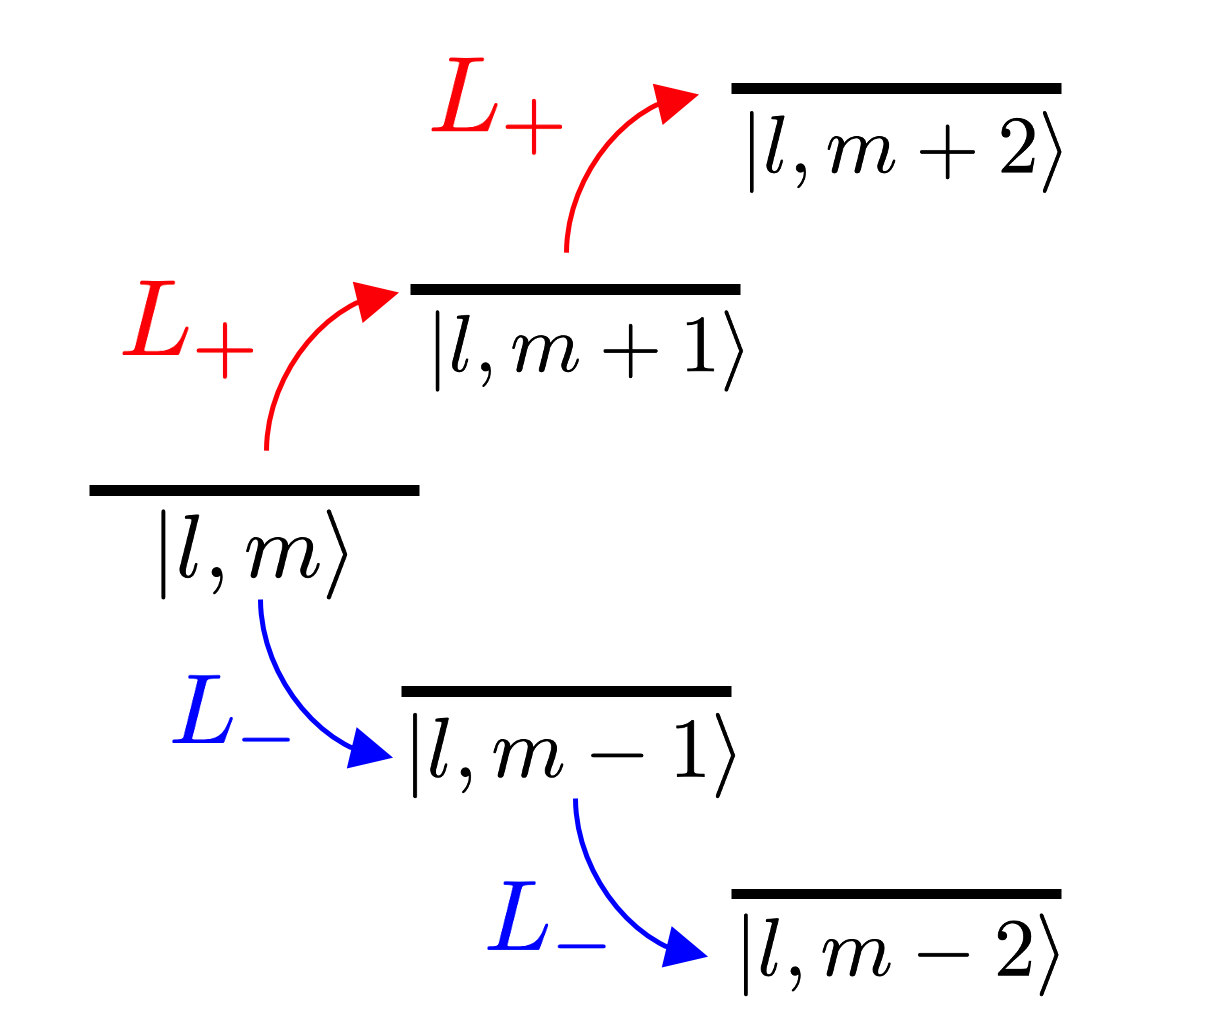
\includegraphics[width=0.35\linewidth]{images/Lowering_Raising_operators.png}
    \caption{Action of the lowering and raising operators $L_-$ and $L_+$; they lower and raise by 1 the quantum number $m$ of the state on which act.}
    \label{fig:lowrai}
\end{figure}
\end{itemize}
Summarizing the results 
\begin{align}
    & L^2 \psi(l,m) = \hbar^2 l(l+1) \psi(l,m) \qquad \text{with} \qquad l \in \frac{\mathbb{N}}{2} \\
    & L_z \psi(l,m) = \hbar m \psi(l,m), \qquad \text{with} \qquad m \in \, \{-l, \, ..., \, +l \}
\end{align}

It is important to notice that these rules follow only from the Lie algebra of the angular momentum operators; by concerning the orbital angular momentum defined in (\ref{eq:Ldef}), it is possible to deduce further restrictions on $l$. Indeed, introducing
\begin{align*}
    r_1 = \frac{r_x+p_y}{\sqrt{2}}, \qquad p_1 = \frac{r_x-p_y}{\sqrt{2}}, \qquad r_2 = \frac{p_x-r_y}{\sqrt{2}} \qquad \text{and} \qquad p_2 = \frac{p_x+r_y}{\sqrt{2}}
\end{align*}
the operator $L_z$ (from (\ref{eq:Li})) becomes
\begin{align*}
        L_z = r_x p_y - r_y p_x = \frac{1}{2}\left(r_1^2 + p_1^2\right) - \frac{1}{2}\left(r_2^2+p_2^2\right).
\end{align*}
It resembles the Hamiltonian of two decoupled harmonic oscillators ($r_1$, $p_1$, $r_1$ and $r_2$ satisfy the same commutation rules) and therefore one can deduce the form of the energy spectrum and write 
\begin{align*}
    L_z \, \psi(l,m) = \hbar m \, \psi(l,m) = \hbar \left[ \left(n_1 +\frac{1}{2}\right) - \left(n_2 + \frac{1}{2}\right)\right] \psi(l,m) = \hbar (n_1-n_2) \, \psi(l,m).
\end{align*}
Since $n_1, n_2 \in \mathbb{N}$, therefore $m \equiv n_1 - n_2 \in \mathbb{N}$ and also $l \in \mathbb{N}$. 

\subsubsection{$L$ in spherical coordinates}

The orbital angular momentum operator can be written in spherical coordinates; indeed, if one introduces three variables 
\begin{align*}
    r \in [0,\infty), \qquad \theta \in [0,\pi) \qquad \text{and} \qquad \varphi \in [0, 2\pi)
\end{align*}
and the versors
\begin{align*}
    \hat{r} = \begin{pmatrix} \sin{\theta} \cos{\varphi} \\ \sin{\theta} \sin{\varphi} \\ \cos{\theta} \end{pmatrix}, \qquad \hat{\theta} = \begin{pmatrix} \cos{\theta} \cos{\varphi} \\ \cos{\theta} \sin{\varphi} \\ -\sin{\theta} \end{pmatrix} \qquad \text{and} \qquad \hat{\varphi} = \begin{pmatrix} -\sin{\varphi} \\ \cos{\varphi} \\ 0  \end{pmatrix},
\end{align*}
the gradient becomes 
\begin{align}
   \vec{\nabla} = \hat{r} \frac{\partial}{\partial r} + \hat{\theta} \frac{1}{r} \frac{\partial}{\partial \theta} + \hat{\varphi} \frac{1}{r \sin{\theta}} \frac{\partial}{\partial\varphi}
   %\label{eq:laplacian_spher}
\end{align}
and $\vec{L}$ can be written starting form (\ref{eq:Ldef})
\begin{align*}
    \vec{L} &= r \, \hat{r} \cross (-i \hbar) \vec{\nabla} = \\
    &= -i\hbar \left( \hat{r} \cross \hat{r} r \frac{\partial}{\partial r} + \hat{r} \cross \hat{\theta} r  \frac{1}{r} \frac{\partial}{\partial \theta} +  \hat{r} \cross \hat{\varphi} r \frac{1}{r \sin{\theta}} \frac{\partial}{\partial\varphi} \right) = \\
    &= -i \hbar \left( \hat{\varphi}  \frac{\partial}{\partial \theta} -  \hat{\theta} \frac{1}{r \sin{\theta}} \frac{\partial}{\partial\varphi} \right). 
\end{align*}
From this expression, one can conclude that the orbital angular momentum operator acts only on a sphere surface because there is no dependence on $r$. 
Also the component of $\vec{L}$ can be expressed in spherical coordinates
\begin{align*}
    L_x = \vec{L} \cdot \vec{x} &= -i \hbar \left( \hat{x} \cdot \hat{\varphi} \frac{\partial}{\partial \theta} - \hat{x} \cdot \hat{\theta} \frac{1}{\sin{\theta}} \frac{\partial}{\partial \varphi}\right) = i\hbar \left( \sin{\varphi} \frac{\partial}{\partial \theta} + \cos{\theta} \cos{\varphi} \frac{\partial}{\partial \varphi} \right), \\
    L_y = \vec{L} \cdot \vec{y} &= -i \hbar \left( \hat{y} \cdot \hat{\varphi} \frac{\partial}{\partial \theta} - \hat{y} \cdot \hat{\theta} \frac{1}{\sin{\theta}} \frac{\partial}{\partial \varphi}\right) = i\hbar \left( -\cos{\varphi} \frac{\partial}{\partial \theta} + \cos{\theta} \cos{\varphi}  \frac{\partial}{\partial \varphi} \right), \\
    L_z = \vec{L} \cdot \vec{z} &= -i \hbar \left( \hat{z} \cdot \hat{\varphi} \frac{\partial}{\partial \theta} - \hat{z} \cdot \hat{\theta} \frac{1}{\sin{\theta}} \frac{\partial}{\partial \varphi}\right) = i\hbar \frac{\partial}{\partial \varphi},
\end{align*}
and similarly for the operators $L_\pm$
\begin{align*}
    L_+ &= L_x + i L_y = i \hbar (\cos{\varphi} + i \sin{\varphi}) \left( \cot{\theta} \frac{\partial}{\partial \varphi} -i \frac{\partial}{\partial \theta} \right) = i\hbar e^{i \varphi} \left( \cot{\theta} \frac{\partial}{\partial \varphi} -i \frac{\partial}{\partial \theta} \right), \\
    L_- &= L_x - i L_y = i \hbar (\cos{\varphi} - i \sin{\varphi}) \left( \cot{\theta} \frac{\partial}{\partial \varphi}+ i \frac{\partial}{\partial \theta} \right) = i\hbar e^{-i \varphi} \left( \cot{\theta} \frac{\partial}{\partial \varphi}+i \frac{\partial}{\partial \theta} \right).
\end{align*}
With these results and by using the relation in (\ref{eq:L2}) it is possible to obtain the expression for $L^2$ in spherical coordinates:
\begin{align*}
    L^2 = -\hbar^2 \left[\frac{1}{\sin{\theta}} \frac{\partial}{\partial \theta} \left( \sin{\theta} \frac{\partial}{\partial \theta} \right) + \frac{1}{\sin^2{\theta}} \frac{\partial^2}{\partial \varphi^2}.  \right]
\end{align*}
If one considers the Laplacian operator
\begin{align}
   \nabla^2 = \frac{1}{r^2} \frac{\partial}{\partial r} \left( r^2 \frac{\partial}{\partial r}\right) + \frac{1}{r^2 \sin{\theta}}  \frac{\partial}{\partial \theta}  \left( \sin{\theta} \frac{\partial}{\partial \theta} \right) + \frac{1}{r^2 \sin^2{\theta}} \frac{\partial^2}{\partial\varphi^2},
   \label{eq:laplacian_spher}
\end{align}
it is possible to notice that it can be written in terms of $L^2$ as
\begin{align*}
    \nabla^2 =  \frac{1}{r^2} \frac{\partial}{\partial r}  r^2 \frac{\partial}{\partial r}+ \frac{L^2}{r^2}. 
\end{align*}
These considerations are useful to obtain an important expression for a generic Hamiltonian, indeed
\begin{align}
    H = \frac{p^2}{2m}+V(\Vec{r}) = -\frac{\hbar^2}{2m} \nabla^2 + V(\Vec{r}) = -\frac{\hbar^2}{2m}\frac{1}{r^2}\frac{\partial}{\partial r} r^2 \frac{\partial}{\partial r} + \frac{L^2}{2m r^2} + V(\vec{r}).
    \label{eq:Hatoms3}
\end{align}
When the potential is a function of just $\abs{\vec{r}}$ ($V(\vec{r}) = V(r)$), $H$ can be decomposed in its radial and angular parts and hence the eigenfunctions $\psi(r,\theta,\varphi)$ can be written as 
\begin{align}
    \psi_{n,l,m}(r,\theta,\varphi) = R_{n,l}(r) \, Y_{l,m}(\theta,\varphi),
    \label{eq:psi_compl}
\end{align}
where $n$ is an additional quantum number which is discussed in the following section. 

\subsubsection{Angular part of $\psi(r,\theta,\varphi)$}

Firstly, consider only the angular part of $H$ in (\ref{eq:Hatoms3}) and search for the functions $Y_{l,m}(\theta,\varphi)$, called \textit{spherical harmonics}, that give the angular distribution of the states $\ket{l,m}$; since $H$ commutes with $L^2$ and $L_z$, $Y_{l,m}(\theta,\varphi)$ are also eigenstates of $L_z$:
\begin{equation*}
    L_z \, Y_{l,m}(\theta,\varphi) = \hbar m Y_{l,m}(\theta,\varphi).
\end{equation*}
Given the expression for $L_z$ in spherical coordinates, the solution can be written in the form
\begin{equation}
    Y_{l,m}(\theta, \varphi) = P_l^m(\theta) e^{im\varphi}, 
\end{equation}
where $P_l^m(\theta)$ is the Legendre polynomial associated to $Y_{l,m}(\theta, \varphi)$. To find the explicit expression of $P_l^m$, one can start from the case $m = l$ and remember that:
\begin{equation*}
     L_+ \, Y_{l,l} = 0 \quad \implies \quad \left( \cot{\theta} \frac{\partial}{\partial \varphi} - i \frac{\partial}{\partial \theta}\right) e^{il\varphi} P_l^l (\theta) = \left( l \cot{\theta} - \frac{\partial}{\partial \theta} \right) P_l^l(\theta)= 0.
\end{equation*}
This is a differential equation which has an unique solution for $l \in \mathbb{N}$:
\begin{equation}
    P_l^l(\theta)=\sin^l{(\theta)}.
\end{equation}
From this expression, one can evaluate all the other spherical harmonics action of the lowering operator reported in (\ref{eq:L-action}):
\begin{equation*}
    Y_{l,m-1}(\theta, \varphi) = \frac{1}{\sqrt{l(l+1)-m(m-1)}} L_- \, Y_{l,m}(\theta, \varphi).
\end{equation*}

\begin{tcolorbox}[breakable, enhanced]
\textbf{Some spherical harmonics} \\
    The first few spherical harmonics are: 
    \begin{itemize}
    \item \textbf{$l = 0$}
    \begin{align*}
        Y_{0,0} &= \sqrt{\frac{1}{4\pi}}
    \end{align*}
    \item \textbf{$l = 1$}
    \begin{align*}
        Y_{1,-1} &= \sqrt{\frac{3}{8\pi}} \sin{\theta} e^{-i\varphi} \\
        Y_{1,0} &= \sqrt{\frac{3}{4\pi}} \cos{\theta} \\
        Y_{1,1} &= -\sqrt{\frac{3}{8\pi}} \sin{\theta)} e^{i\varphi} 
        \end{align*}
      \item  \textbf{$l = 2$}
        \begin{align*}
        Y_{2,-2} &= \frac{1}{4} \sqrt{\frac{15}{2\pi}} \sin^2{\theta} e^{-2i\varphi} \\
        Y_{2,-1} &= \frac{1}{2} \sqrt{\frac{15}{2\pi}}\sin{\theta} \cos{\theta} e^{-i\varphi} \\
         Y_{20} &= \frac{1}{4} \sqrt{\frac{5}{\pi}}  (3 \cos^2{\theta}-1) \\
        Y_{2,1} &= -\frac{1}{2} \sqrt{\frac{15}{2\pi}}\sin{\theta} \cos{\theta} e^{i\varphi} \\
        Y_{2,2} &= \frac{1}{4} \sqrt{\frac{15}{2\pi}} \sin^2{\theta} e^{2i\varphi}
    \end{align*}
    \end{itemize}
   The normalization condition is:
    \begin{equation*}
        \int Y^*_{l,m} \, Y_{l',m'} \, \sin{\theta} \, d\theta d\varphi = \delta_{l,l'} \delta_{m,m'}.
    \end{equation*}
    The solutions with $l=0$ are called \textit{s orbitals} (which stands for ``sharp", as they have no degeneracy), those with $l=1$ are called \textit{p orbitals} (which stands for ``principal", as they correspond to the brightest lines in the spectra) and those with $l=2$ are called \textit{d orbitals} (which stands for ``diffuse", due to their high degeneracy). 
\end{tcolorbox}

\subsubsection{Radial part of $\psi(r,\theta,\varphi)$}

The function $\psi_{n,l,m}(r,\theta,\varphi)$, as written in (\ref{eq:psi_compl}), comprehends also a radial part, which depends on the quantum numbers $n$ and $l$. In order to study it, consider the Hamiltonian $H$ in (\ref{eq:Hatoms3}) and take into account the fact that $Y_{l,m}$ is an eigenstate of $L^2$ with eigenvalue $\hbar^2 l(l+1)$; with these consideration, the Schr\"odinger equation can be written in the form:

\begin{align*}
    H \psi_{n,l,m}(r,\theta,\varphi) &= \left(-\frac{\hbar^2}{2m}\frac{1}{r^2}\frac{\partial}{\partial r}\left(r^2 \frac{\partial}{\partial r}\right) + V(r)+ \frac{\hbar^2 l(l+1)}{2m r^2}\right)Y_{l,m}(\theta,\varphi) R_{n,l}(r) = \\
    &= E \, \psi_{n,l,m}(r,\theta,\varphi).
\end{align*}

It is customary to introduce a function $P_{n,l}(r) = r \, R_{n,l}(r)$ and to obtain a modified radial Schr\"odinger equation 
\begin{equation}
    \left(-\frac{\hbar^2}{2m} \frac{\partial^2}{\partial r ^2}+ V_\text{eff}(r)\right) P_{n,l}(r)= E \, P_{n,l}(r),
    \label{eq:eqP}
\end{equation}
where the $V_\text{eff}$ contains both the radial potential and the centrifugal effect given by orbital angular momentum.

\subsection{Spectrum of the Hydrogen atom}

Equation (\ref{eq:eqP}) is a one-dimensional differential equation and it is similar to the one obtained for the Hydrogen atom if 
\begin{align}
    V_\text{eff}(r) = \frac{\hbar^2 l(l+1)}{2 m r^2} - \frac{Z_\text{eff} e^2}{4 \pi \epsilon_0 r},
\end{align}
in which $Z_\text{eff}$ represents the charge (in units of $e$) of the attractor part and this case is $Z_\text{eff} = 1$. The behaviour of this potential is reported in figure \ref{fig:eff_potential}, while the solutions of the discussed Schr\"odinger equation constitute the energy levels reported in the spectrum in figure (\ref{fig:hydro_spectrum}).

\begin{figure}[h!]
\centering
    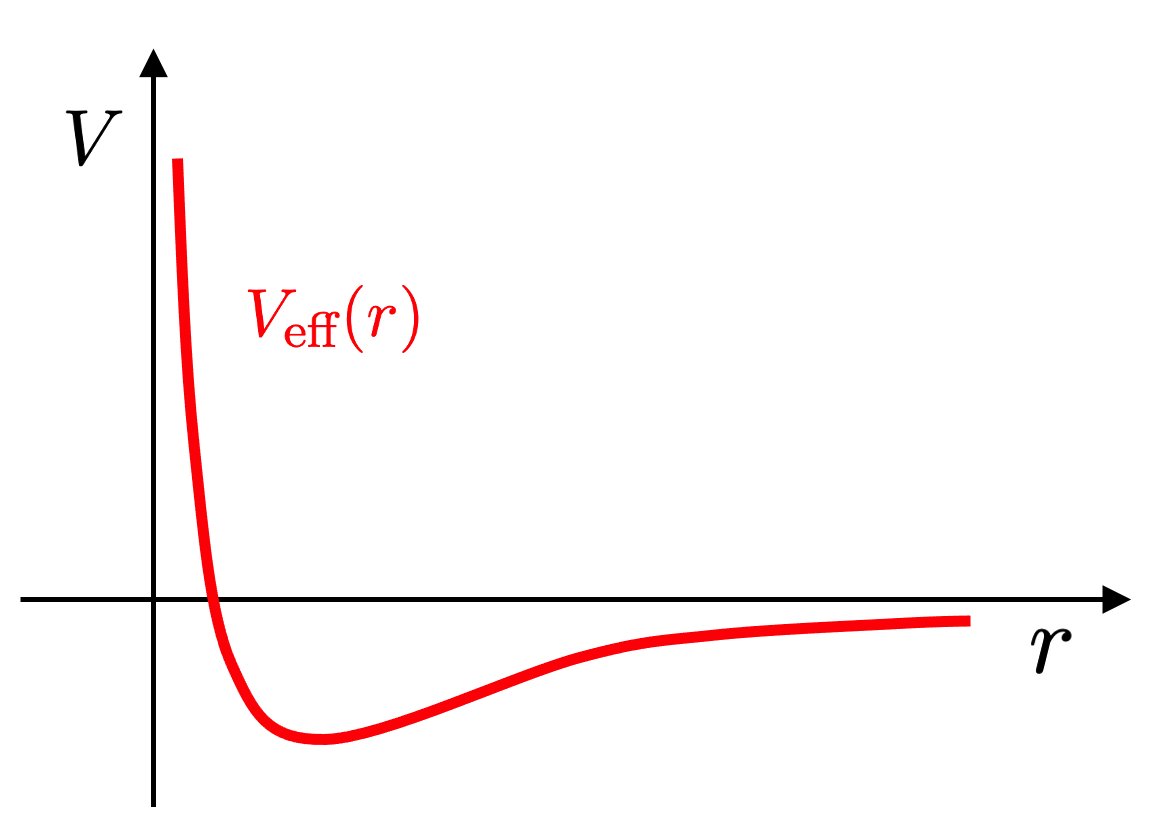
\includegraphics[width=0.45\linewidth]{images/Effective_potential.png}
    \caption{Behaviour or the effective potential; the repulsive part for low values of $r$ is associated to the angular component, the attractive part for high values of $r$ is associated to the electric part.}
    \label{fig:eff_potential}
\end{figure}

\begin{figure}[h!]
\centering
    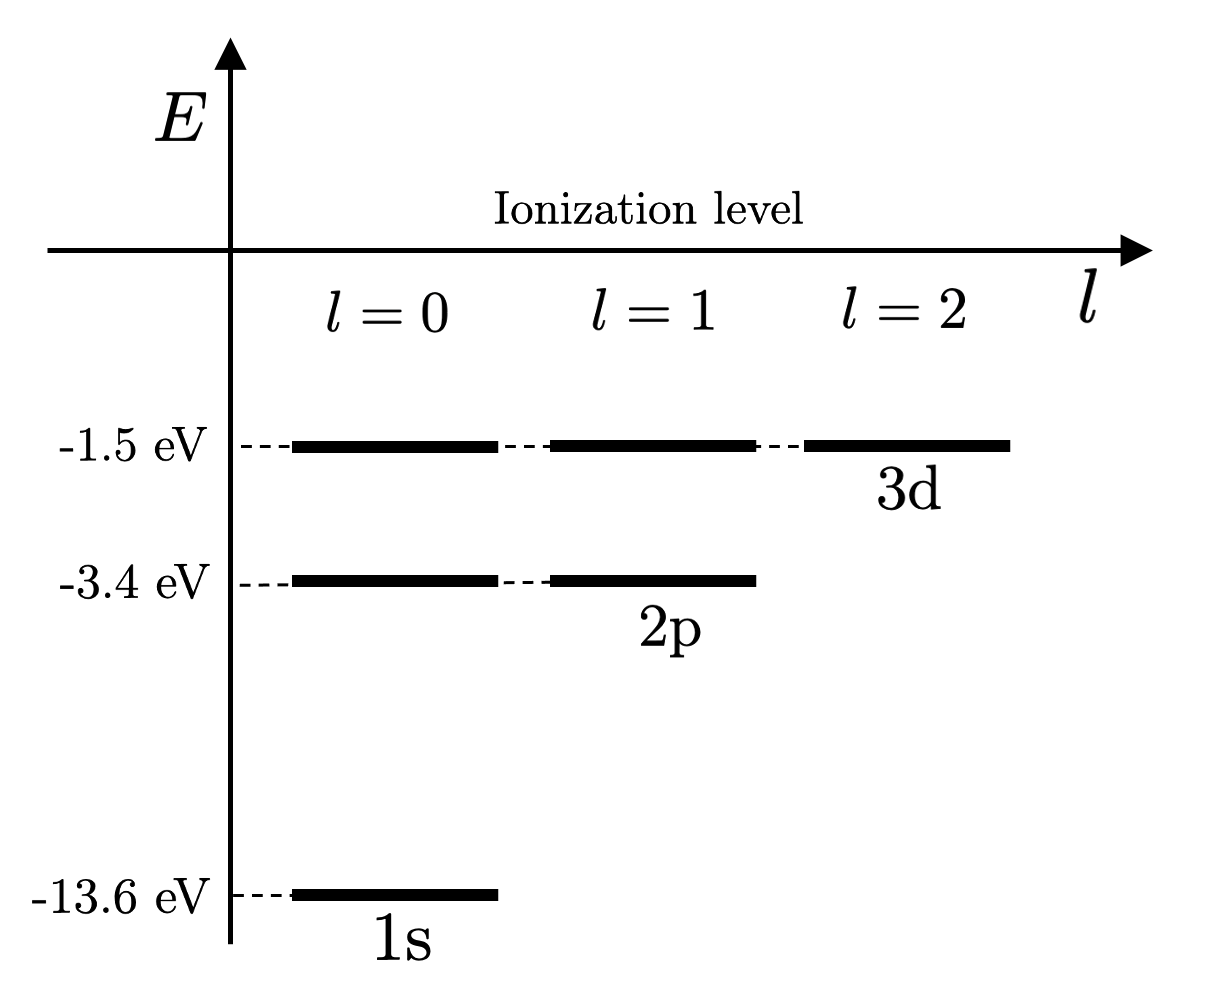
\includegraphics[width=0.5\linewidth]{images/Hydrogen_spectrum.png}
    \caption{First levels of the Hydrogen electron spectrum with the relative energies and orbital names.}
    \label{fig:hydro_spectrum}
\end{figure}

\subsection{Alkali atoms}

\begin{figure}[t]
\centering
    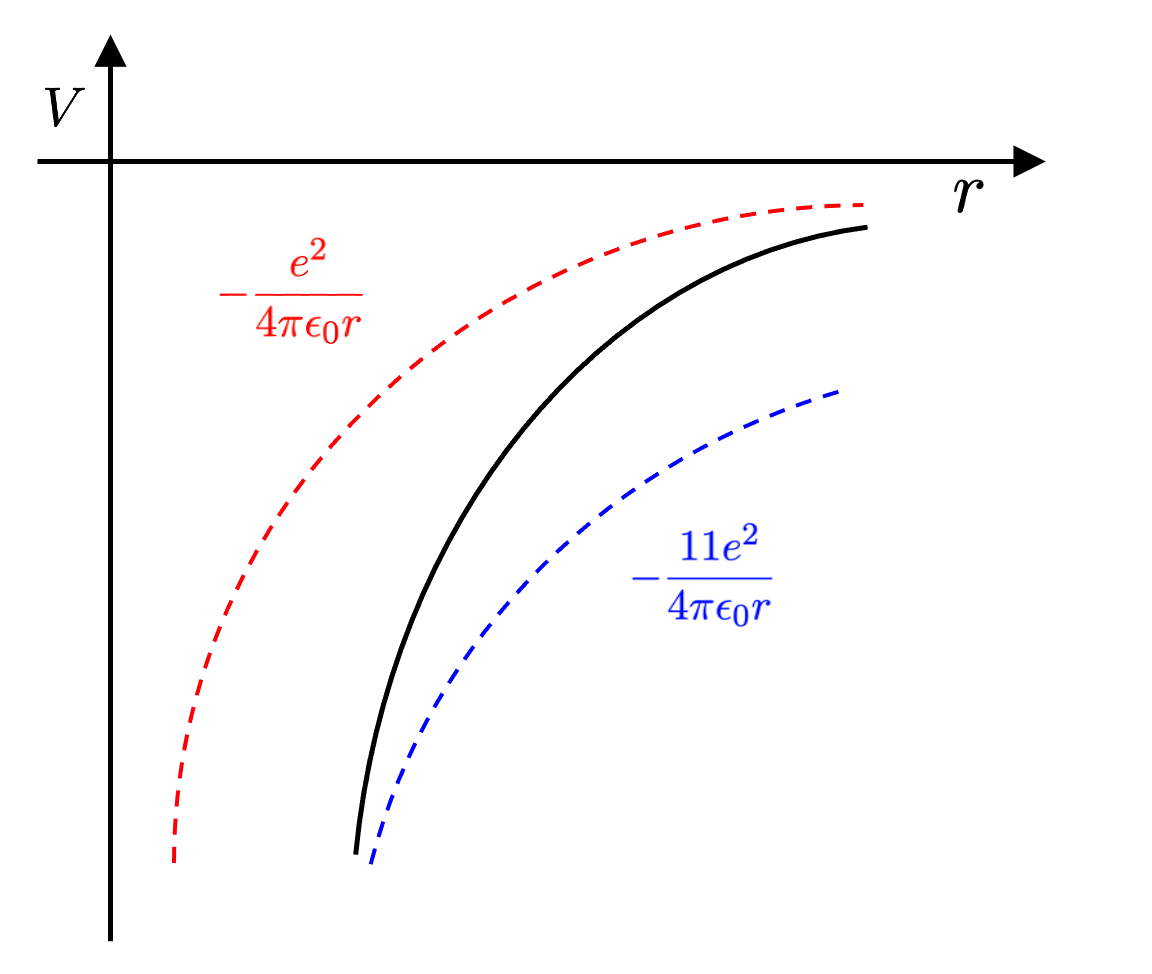
\includegraphics[width=0.58\linewidth]{images/Alkali_potential.png}
    \caption{Potential felt by the outer electron of a Sodium atom; for small distances an additional attractive term with respect to the Hydrogen potential is present and the total potential is shifted down, while for large distances the electron sees only the potential of a Hydrogen core.}
    \label{fig:pot_Alkali}
\end{figure}

\begin{figure}[b]
\centering
    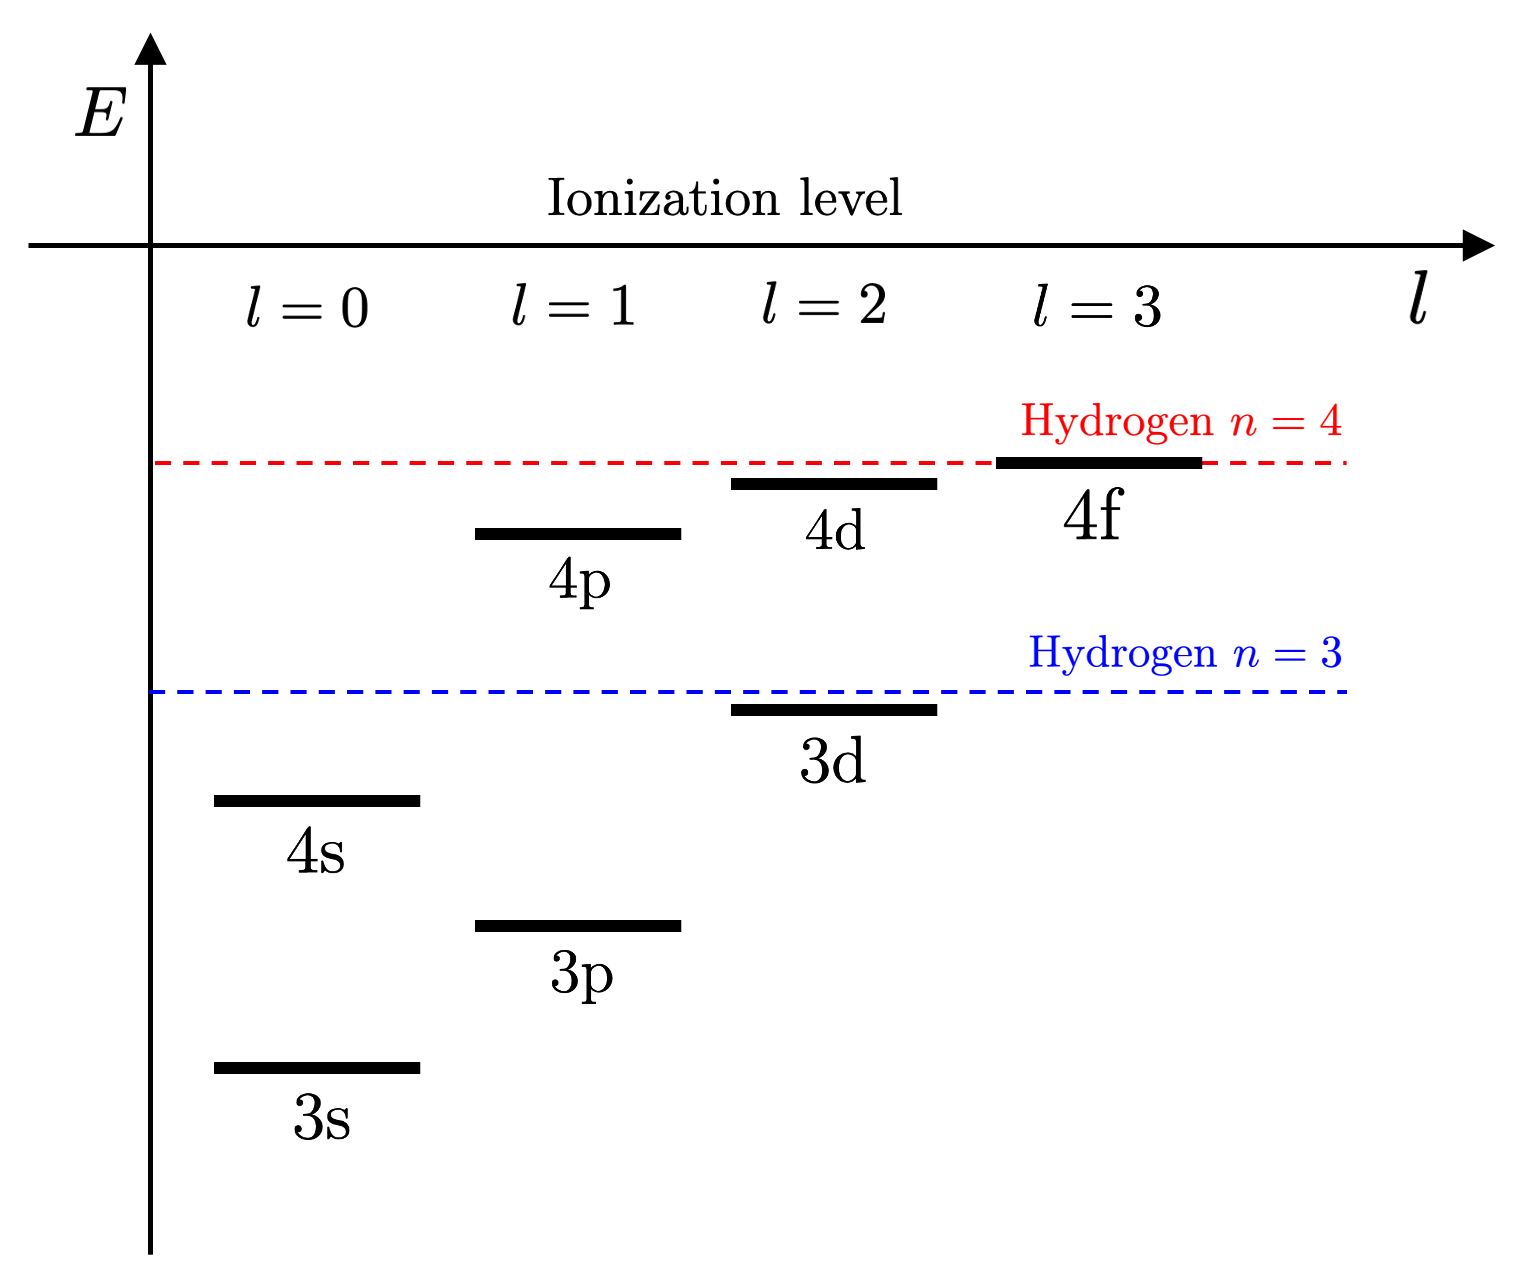
\includegraphics[width=0.61\linewidth]{images/Alkali_spectrum.png}
    \caption{First levels of the Sodium electron spectrum with the relative energies and orbital names; also the reference energies from the Hydrogen spectrum are reported.}
    \label{fig:alkali_spectrum}
\end{figure}


Hydrogen atoms are not used in everyday applications because they are light and volatile at temperatures little higher than the absolute zero. To avoid this, heavier atoms, like Alkali and in particular $^{11} \text{Na}_{\sim 22}$, are used. 

\noindent The Hamiltonian associated to these atoms is
\begin{equation}
    H_\text{Alkali} = \sum_{j} \left( - \frac{\hbar^2}{2m} \nabla_j^2 - \frac{Ze^2}{4 \pi \epsilon_0 \left| \Vec{r}_j\right|}\right) + \sum_{j\neq j'} \frac{e^2}{4 \pi \epsilon_0 \left| \Vec{r}_j - \Vec{r}_{j'}\right|}, 
    \label{eq:alkali_hamiltonian}
\end{equation}
where the summations are performed over the electrons. It can be be rewritten in many better ways, through some approximations. One could express $H_\text{Alkali}$ using the \textit{Hartree-Fock approximation}, but the entanglement information would be lost, due to the fact that this approximation provides the use of the \textit{mean field}.

Another possibility is the \textit{Shell model approximation}, which is a harsher approximation with respect to the previous one: the idea is that every electron sees only the core screened by the previous electrons. The behaviour of this potential for the outer electron of Sodium atom is reported in figure \ref{fig:pot_Alkali}. This model also gives a good explanation of the energy shift for atomic orbitals observed in alkali atoms with respect to the Hydrogen levels (figure \ref{fig:alkali_spectrum}); indeed, shifting momentarily towards a semi-classical picture with the electron as a proper particle orbiting around the nucleus, one could imagine that two processes take place:
\begin{itemize}
    \item as the electron gets closer to the nucleus, the electrostatic potential is stronger and the energy shift more pronounced;
    \item electrons with higher $l$ number experience a stronger centrifugal potential, bringing them farther away from the nucleus, resulting in a weaker electrostatic attraction and smaller energy shift.
\end{itemize}



\section{Interaction of Alkali atoms with light}
The interaction between charged particles and the electromagnetic field is governed by the Lorentz force $\Vec{F_L}=q(\Vec{E}+\Vec{v}\cross\Vec{B})$. The Lagrangian of a system where this is the only force in play is 
\begin{equation*}
    L(\Vec{r}, \Dot{\Vec{r}}, t)=\frac{1}{2} m \Dot{r}^2 + q \Dot{\Vec{r}}\cdot\Vec{A}- q \phi,
\end{equation*}
where the last part is equivalent to $J_\mu A^\mu$ in relativistic notation. Moving to the Hamiltonian view, since the canonical momentum is defined as 
\begin{equation*}
    p_i=\frac{\partial L}{\partial \Dot{\Vec{r}}} \qquad \implies \qquad \Vec{p}=m\Dot{\Vec{r}}+q\Vec{A}. 
\end{equation*}
The Hamiltonian in this \textit{minimal coupling} case can thus be written as 
\begin{equation}
    H= \frac{(\Vec{p}-q\Vec{A})^2}{2m}+q\phi, 
    \label{eq:Hatomlight}
\end{equation}
where both the part relative to the motion of the atom and the one associated to the interaction with light are present. 

\subsection{Power-Zienau transformation}

When using light at wavelengths such that $k^{-1}\gg a_0$ (where $a_0$ is the Bohr radius, i.e. the average of the electron-nucleus distance), as is the case with visible light, 
\begin{align*}
    \Vec{A}(\Vec{r}, t) \qquad \longrightarrow \qquad \Vec{A}({0}, t).
\end{align*}
This means that if the light wavelength is much larger than the interaction region (approximated by $a_0$), the vector potential is expected to vary little enough to be approximated with its central value. Within this approximation, which is called \textit{long-wavelength approximation}, $\Vec{A}$ commutes with momentum $\vec{p}$, since it no longer depends on position, i.e.
\begin{align*}
    \left[\vec{A}(\vec{r}),\, \vec{p} \right] \neq 0 \qquad \qquad  \left[\vec{A}(0),\, \vec{p} \right] = 0.
\end{align*}

% Power-Zienam transformation
The atom-light Hamiltonian (\ref{eq:Hatomlight}) can be rewritten by defining an unitary operator, the \textit{Power-Zienau transformation}
\begin{equation*}
    T = \exp{-\frac{i}{\hbar} q \, \Vec{r}\cdot\Vec{A}(0)}
\end{equation*}
and by using the using Hadamard's lemma
\begin{align*}
    e^{-S} \, B \,e^S = B+[S,B]+\frac{1}{2} [S,[S,B]]+...~
\end{align*}
to evaluate $H_{AL}'= T \, H_{AL} \, T^\dagger$. The first step consists of evaluating
\begin{align*}
    \Vec{p}\,'&=T\,\Vec{p}\,\,T^\dagger=\Vec{p}-\frac{i}{\hbar} q \left[\Vec{r}\cdot\Vec{A}(0), \, \Vec{p}\right] - \frac{q^2}{2\hbar^2} \left[\Vec{r}\cdot\Vec{A}(0),\left[\Vec{r}\cdot\Vec{A}(0),\Vec{p}\right]\right]+... = \\
    &=\Vec{p}-\frac{i}{\hbar} q \Vec{A}(0) \, \left[\Vec{r},\,\Vec{p}\right]=\Vec{p}+q\Vec{A},
\end{align*}
given that $[\Vec{r}, \, \Vec{p}]=i\hbar \mathbb{1}$ and thus all higher-order commutators are null. Therefore, 
\begin{equation*}
    T (\Vec{p}-q\Vec{A})^2 T^\dagger = T (\Vec{p}-q\Vec{A}) T^\dagger \, T (\Vec{p}-q\Vec{A}) T^\dagger = (\vec{p} + q \vec{A} - q \vec{A}) \cdot \vec{p} = p^2,
\end{equation*}
because $\vec{A}'(0) = T \vec{A}(0) T^\dagger = \vec{A}(0)$. Since $\phi'(\vec{r}) = T \phi(\vec{r}) T^\dagger = \phi(\vec{r})$, the final expression for $H_{AL}$ is
\begin{align}
    H'_{AL} = T H_{AL} T^\dagger = \frac{p^2}{2m} + q \phi. 
\end{align}

\subsection{Dipole approximation}
\label{dipole}

The same transformation can be applied to the Hamiltonian of the electromagnetic field $H_\text{light} \equiv H_{EM}$, treated in the previous chapter. In particular, using the Hadamard's relation 
\begin{align*}
    H'_{EM} &= T H_{EM} T^\dagger = \\
    &= H_{EM} - \frac{i}{\hbar} q \left[\vec{r} \cdot \vec{A}(0), \, H_{EM} \right] - \frac{q^2}{2\hbar^2} \left[ \vec{r} \cdot \vec{A}(0), \, \left[  \vec{r} \cdot \vec{A}(0), H_{EM} \right]\right] + ... = \\ 
    &= H_{EM} - \frac{i}{\hbar} {r_i} \left[ {A_i}(0), H_{EM}\right] - \frac{q^2}{2\hbar^2} r_i \, r_j \left[ A_i(0), \left[ A_j(0), H_{EM} \right] \right] + ..., 
\end{align*}
where the repeated indexes indicate a summation over the three components. Introducing the \textit{dipole operator} $\Vec{d}\equiv q\Vec{r},$ $H'_{EM}$ becomes 
\begin{equation}
    H'_{EM} = H_{EM} - \frac{i}{\hbar} d_i [A_i(0), H_{EM}]- \frac{1}{2\hbar^2} d_i d_j [A_i(0),[A_j(0), H_{EM}]]+ ...
    \label{eq:Hem1}
\end{equation}
The commutator in the previous expression is evaluated inserting the relation (\ref{eq:potvec}) for $\Vec{A}$ with $u(\Vec{r} = 0) \approx 1$:
\begin{align*}
    \left[\Vec{A}(0), H_{EM} \right] &= \sum_{\vec{k},\lambda} \sqrt{\frac{\hbar}{2 \varepsilon_0 \omega_k}} \frac{\vec{\epsilon}_\lambda}{\sqrt{V}} \left[ \left(a_{\vec{k},\lambda} + a_{\vec{k},\lambda}^\dagger\right), H_{EM}\right] = \\
    &= \sum_{\vec{k},\lambda} \sqrt{\frac{\hbar}{2 \varepsilon_0 \omega_k}} \frac{\vec{\epsilon}_\lambda}{\sqrt{V}} \left[ \left(a_{\vec{k},\lambda} + a_{\vec{k},\lambda}^\dagger\right), \sum_{\vec{k}',\lambda'} \hbar \omega_{k'} a_{\vec{k}',\lambda}'^\dagger a_{\vec{k}',\lambda'} \right] = \\
    &= \sum\limits_{\substack{\Vec{k},\lambda, \\ \Vec{k}', \lambda'}}
    \sqrt{\frac{\hbar}{2\epsilon_0\omega_k}} \frac{\Vec{\epsilon}_\lambda}{\sqrt{V}} \hbar\omega_{k'} \left(\left[a_{\Vec{k},\lambda}^\dagger, n_{\Vec{k'},\lambda'}\right]+\left[a_{\Vec{k},\lambda}, n_{\Vec{k'},\lambda'}\right]\right)=\\
    &=\hbar \sum_{\Vec{k}, \lambda} \sqrt{\frac{\hbar\omega_k}{2\epsilon_0}}~ \frac{\Vec{\epsilon}_{\Vec{k}}}{\sqrt{V}} \left(a_{\Vec{k},\lambda}-a_{\Vec{k},\lambda}^\dagger\right)= -i\hbar \Vec{E}(0),
\end{align*}
where the commutators are evaluated as 
\begin{align*}
    \left[a_{\Vec{k},\lambda}^\dagger, n_{\Vec{k'},\lambda'}\right] &= -a_{\vec{k},\lambda}^\dagger \delta_{\vec{k},\vec{k}'} \delta_{\lambda,\lambda'} \\
    \left[a_{\Vec{k},\lambda}, n_{\Vec{k'},\lambda'}\right] &= a_{\vec{k},\lambda} \delta_{\vec{k},\vec{k}'} \delta_{\lambda,\lambda'}
\end{align*}
Then (\ref{eq:Hem1}) becomes 
\begin{align}
    H'_{EM} = H_{EM} - d_i \, E_i(0) - \frac{i}{2 \hbar} d_i d_j \left[ A_i(0), E_j(0)\right] \equiv H_{EM} - \vec{d} \cdot \vec{E}(0) + H_{dd}. 
\end{align}
\\
%where other terms vanish since $[A_i,E_j] = 0$ for $i \neq j$ because 
%\begin{align*}
%    [\Vec{A},\Vec{E}] \propto \left[a_{\Vec{k},\lambda} + a_{\Vec{k},\lambda}^\dagger, a_{\Vec{k'},\lambda'}-a_{\Vec{k'},\lambda'}^\dagger\right] \sim -2 \left[a_{\Vec{k},\lambda}, a_{\Vec{k},\lambda}^\dagger\right] \delta_{\Vec{k}, \Vec{k'}}\delta_{\lambda, \lambda'} \sim -2 \delta_{\Vec{k}, \Vec{k'}}\delta_{\lambda, \lambda'}
%\end{align*}
%is no longer dependent on the field operators, the higher commutators are all zero;  moreover, the second term only operates on the atom degrees of freedom via the dipole operators, resulting in a shift of the atom levels.

The complete Hamiltonian which takes into account the light and the light-matter interaction contributions after the considered transformation is 
\begin{equation}
    H = \frac{p^2}{2m}+ q\phi +H_{dd} + H_{EM} - \Vec{d}\cdot\Vec{E}(0) \equiv H_\text{atom} + H_\text{light} + H_\text{atom-light}
    \label{eq:Hamfin}
\end{equation}
The first three terms define the total atom Hamiltonian, whose eigenstates are written as $\ket{n,l,m}$, the fourth is the light contribution, with eigenstates given by the Fock states, and the last is the first-order approximation for the atom-light interaction Hamiltonian. Higher orders can be obtained using further terms in the multipole expansion for $\Vec{A}$, i.e.
\begin{align*}
    \Vec{A}(\Vec{r}) = \Vec{A}(\Vec{0})+ r_i \frac{\partial}{\partial x_i} \Vec{A}+\frac{1}{2} r_i r_j \frac{\partial^2}{\partial x_i \partial x_j} \Vec{A}+ ... 
\end{align*}

\subsection{Selection rules}

Some considerations can be done about the dipole operator $\vec{d} = q \vec{r}$ which enters in the Hamiltonian for light-atom interaction. 

\subsubsection{Diagonal elements}
Under the \textit{parity transformation} $\Tilde{R}$ defined as
\begin{align*}
    \Tilde{R}\,\psi(x,y,z)&=\psi(-x, -y, -z) \\
    \Tilde{R}\psi(r, \theta, \varphi)&=\psi(r, \pi-\theta, \pi+\varphi),
\end{align*}
with $\Tilde{R}^\dagger=\Tilde{R}^{-1}=\Tilde{R}$, one has
\begin{align*}
    \Tilde{R}\, \Vec{r} \, \Tilde{R}^\dagger =-\Vec{r} \qquad &\Longleftrightarrow \qquad \{ \Tilde{R},\,  \vec{r} \} = 0, \\
    \Tilde{R}\, \Vec{p} \, \Tilde{R}^\dagger =-\Vec{p} \qquad &\Longleftrightarrow \qquad \{ \Tilde{R}, \, \vec{p} \} = 0, \\
     \Tilde{R}\, \Vec{L} \, \Tilde{R}^\dagger =\vec{L} \qquad &\Longleftrightarrow \qquad [ \Tilde{R}, \, \vec{p} ] = 0. \\
\end{align*}
Therefore, $\vec{L}$, $L^2$ and $L_z$ share the eigenbasis $\ket{n,l,m}$; in particular, the eigenvalues for $\Tilde{R}$ are 
\begin{align}
    \Tilde{R}\ket{n,l,m} =  (-1)^l \ket{n,l,m} \equiv e^{i \phi_{l,m}} \ket{n,l,m}
\end{align}
Therefore,
\begin{align*}
    \bra{n,l,m}\Vec{r}\ket{n,l,m} &= \bra{n,l,m} \Tilde{R}^\dagger \Tilde{R}  \Vec{r} \ket{n,l,m} = \\
    &= - \left( \bra{n,l,m} \tilde{R}^\dagger \right) \vec{r} \left( \tilde{R} \ket{n,l,m}\right) =\\
    &= -\bra{n,l,m} \vec{r} \ket{n,l,m}, 
\end{align*}
from which one deduces that the diagonal elements must all be zero.
\begin{equation*}
    \bra{n,l,m}{\Vec{r}}\ket{n,l,m}=0.
\end{equation*}

\subsubsection{Selection rules on $l$}
From the canonical commutators one can derive the identity
\begin{equation*}
    \left[L^2,\left[L^2, \vec{r}\right]\right]=2\hbar^2 \bigl\{\vec{r}, L^2\bigr\}.
\end{equation*}
Multiplying this by $\bra{n_1,l_1,m_1}$ on the left and by $\ket{n_2,l_2,m_2}$ on the right of both sides and bringing everything to the left one gets:
\begin{align*}
    \hbar^4\Bigl((l_1(l_1+1))^2-2l_1(l_1+1)l_2(l_2+1)+(l_2(l_2+1))^2~+\\ 
    -~2l_1(l_1+1)-2l_2(l_2+1)\Bigr)\bra{n_1,l_1,m_1}\Vec{r}\ket{n_2,l_2,m_2} = 0,
\end{align*}
which can be factorized in
\begin{equation*}
    (l_1-l_2+1)(l_1-l_2-1)(l_1+l_2)(l_1+l_2+2)\bra{n_1,l_1,m_1}\Vec{r}\ket{n_2,l_2,m_2} = 0.
\end{equation*}
The last two parenthesis are irrelevant since they can not be null, hence from the first two one has that the only case in which the matrix element can be nonzero is when $\Delta l= l_1 - l_2 =\pm1$. This is a necessary, not sufficient, condition.

\subsubsection{Selection rules on $m$}
In order to obtain a similar relation for the quantum number $m$, one can assume that the electric field is along the $z-$axis and two cases are considered: 
\begin{itemize}
    \item \textbf{Case $\vec{\epsilon} \parallelslant \hat{z}$} \\
    Since $[L_z, r_z]=0$, one immediately gets
    \begin{equation*}
    \bra{n_1,l_1,m_1}[L_z,\Vec{r}]\ket{n_2,l_2,m_2} = 
        0 = \hbar(m_1-m_2)\bra{n_1,l_1,m_1}\Vec{r}\ket{n_2,l_2,m_2} \;\;.
    \end{equation*}
    Thus the matrix element can be nonzero when $\Delta m = m_1 - m_2 =0$. 
    \item \textbf{Case $\vec{\epsilon} \perp \hat{z}$} \\
    Since $[L_z, r_x ]= i\hbar y$ and $[L_z, r_y]=-i\hbar x$, which implies $[L_z, x\pm iy]=\pm\hbar(x\pm iy)$, one gets
    \begin{align*}
        \bra{n_1,l_1,m_1} \left( [L_z, x\pm iy] \mp \hbar(x\pm iy) \right) \ket{n_2,l_2,m_2} = 0
    \end{align*}
    from which
    \begin{align*}
        \hbar(m_1-m_2-1)\bra{n_1,l_1,m_1}(x+iy)\ket{n_2,l_2,m_2} &= 0, \\
        \hbar(m_1-m_2+1)\bra{n_1,l_1,m_1}(x-iy)\ket{n_2,l_2,m_2} &= 0.
    \end{align*}
    Thus the matrix element can be null when the coefficients are null, hence $\Delta m = m_1 - m_2 = \pm 1$. It can be shown that the $+1$ case corresponds to left-handed circularly polarized light, while the $-1$ case corresponds to right-handed light.
\end{itemize}

An example of the application of this selection rules is given in figure (\ref{fig:sodium_spectrum}), in which the allowed transitions for the lowest level of Sodium spectrum are reported.  

\begin{figure}[h]
\centering
    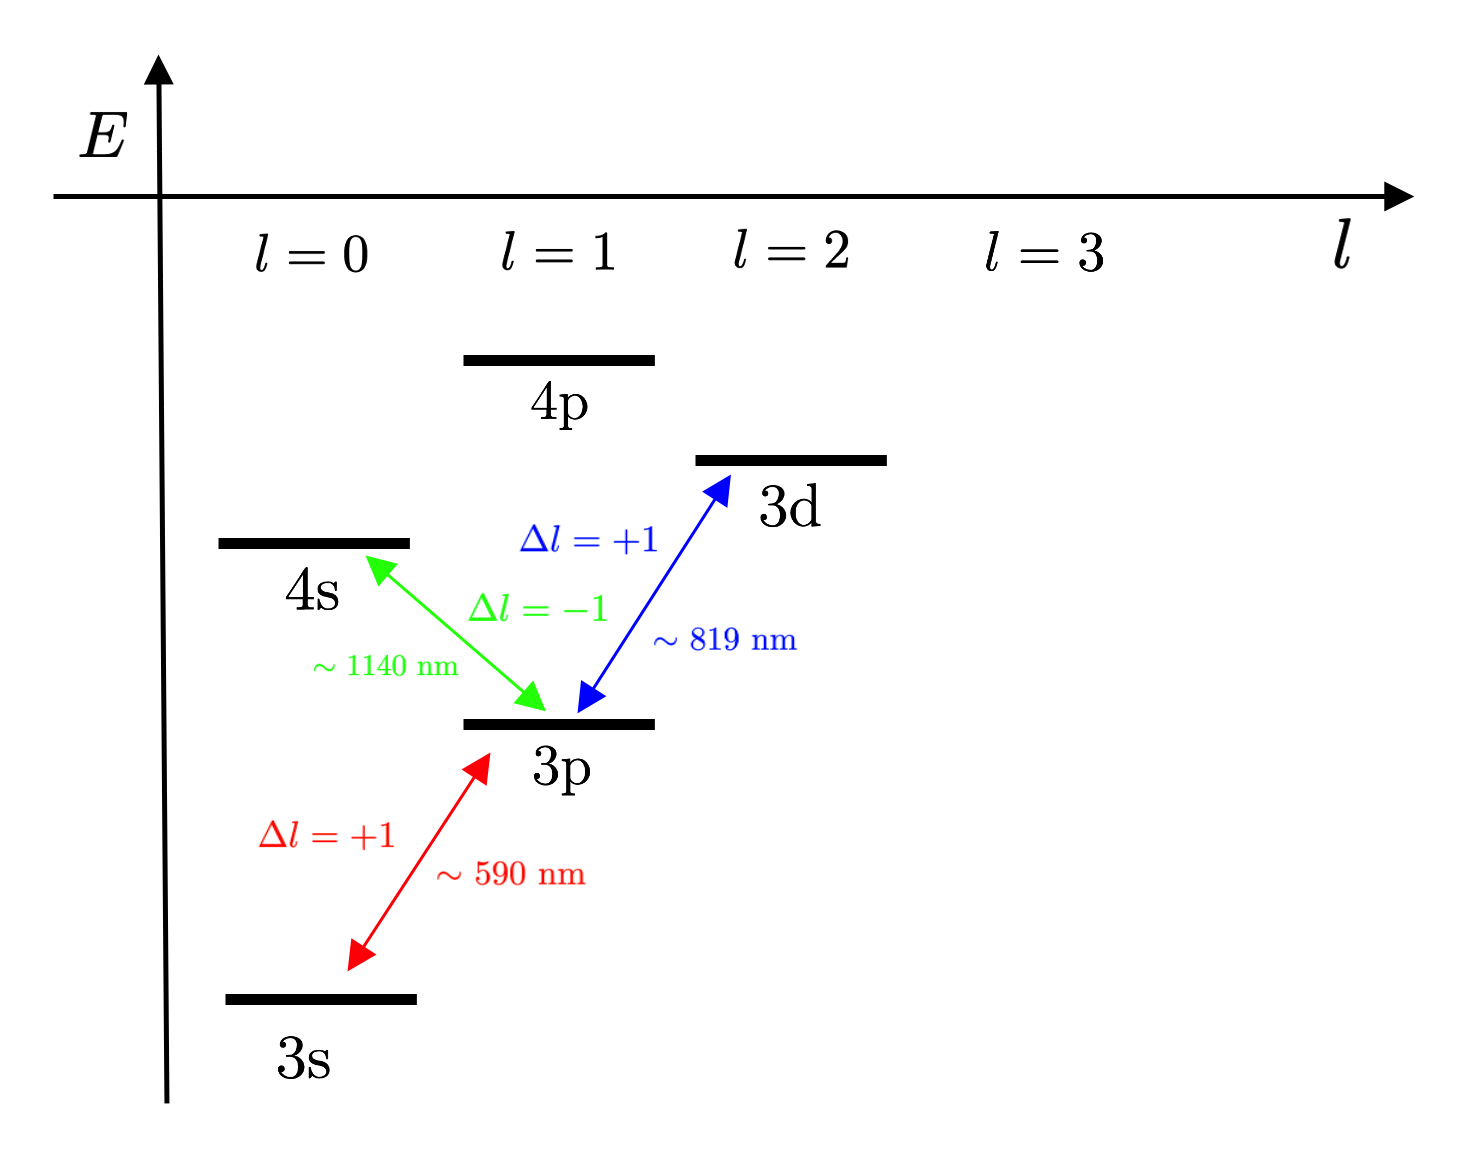
\includegraphics[width=0.7\linewidth]{images/Sodium_transition.png}
    \caption{First levels of the Sodium electron spectrum with the allowed transitions and the relative wavelengths.}
    \label{fig:sodium_spectrum}
\end{figure}





